\section{Análise e Projeto}

\subsection{Visão Geral}

Tal como nos foi apresentado no enunciado, o nosso trabalho era implementar a função $\sum\limits_{i=0}^{n-1} x^2$ em lógica binária. Na figura~\ref{fig:outside} abaixo é possível visualizar o diagrama externo do sistema.

\begin{infoclean}
    Não considere a descrição de $x_i$ concebida mais à frente neste relatório. Considere apenas que é um novo valor de $x$ introduzido.
\end{infoclean}

\begin{figure}[H]
    \centering
    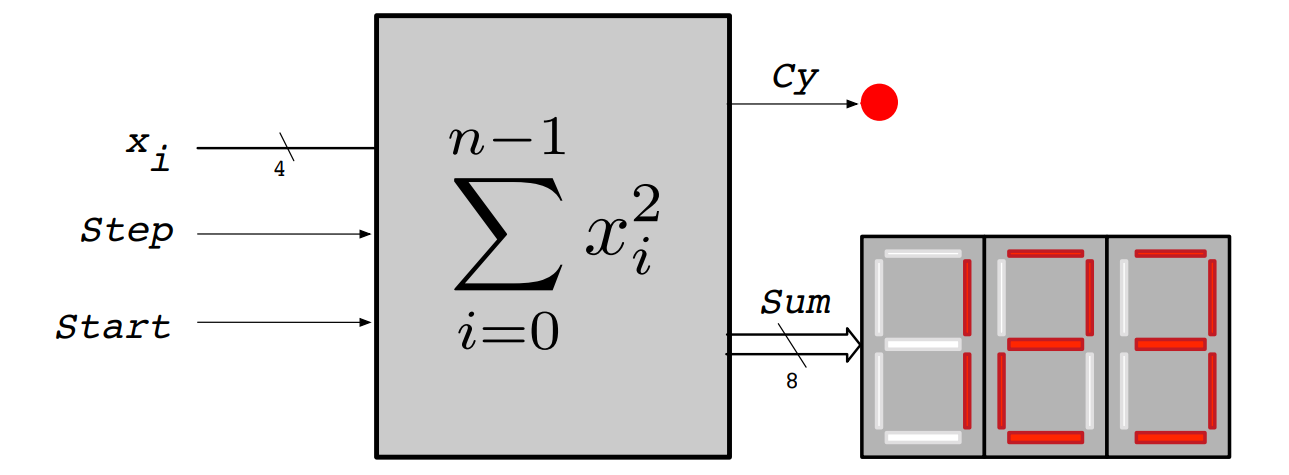
\includegraphics[scale=.3]{Análise e Projeto/Enunciado.png}
    \caption{Diagrama externo do sistema (dado pelo enunciado)}\label{fig:outside}
\end{figure}

Para a conceção deste trabalho, desenvolvemos os dois módulos (Controlador e Caminho de Dados), tal como foi mencionado no enunciado.
Durante a fase de planeamento do projeto, conseguimos simular quatro soluções distintas, cada uma com as suas vantagens e desvantagens (as quais iremos demonstrar à frente). Ao implementar o projeto, optámos pela solução que, na nossa opinião, é a mais adequada.

\subsection{Arquitetura do Sistema}

A arquitetura do sistema é composta por dois módulos principais já mencionados: Caminho de Dados e Controlador. Estes módulos comunicam entre si para garantir o correto funcionamento do sistema e a execução das operações de forma sincronizada.

O Caminho de Dados realiza os cálculos principais do sistema, como o cálculo do quadrado dos números naturais e a soma acumulada dos quadrados. Ele é composto por sub-módulos, como o Quadrado e o Acumulador, projetados para executar funções específicas de maneira eficiente, as quais iram ser demonstradas mais à frente.

O Controlador, por sua vez, descodifica as entradas \textit{Step} e \textit{Reset} e envia os sinais resultantes para o caminho de dados. Este módulo também recebe as saídas do Caminho de Dados.

Como é possível observar na figura~\ref{fig:arq_sist}, estes dois módulos trabalham juntos: o Caminho de Dados realiza os cálculos, enquanto o Controlador gere os sinais. Nos capítulos seguintes, serão descritas as funcionalidades internas de cada módulo e suas interações.

\begin{infoclean}
    Note que, para todos os componentes deste relatório, o \gls{clock} será sempre omitido na representação. Tenha assim em conta, que componentes como \glspl{ffd} e registos (componentes dependentes de \gls{clock}) não são representados com a sua entrada de sinal de \gls{clock}. Note também, que a saída Out é equivalente a três saídas em hexadecimal. Neste relatório omitimos a conversão para hexadecimal mas, ainda assim, considere a sua utilização.
\end{infoclean}

\begin{figure}[H]
    \centering
    \begin{tikzpicture}[node distance=4cm]


    \begin{scope}[scale=0.8, transform shape]
        % Controller
        \node[module, minimum width = 2cm, minimum height = 7.5cm] (controller) {Controller};
        \node[io, label={[yshift=.5cm]left:Step}, yshift = .83*4cm] (step_i) at (controller.west) {};
        \node[io, label={[yshift=.5cm]left:Start}, yshift = .83*3cm] (start_i) at (controller.west) {};
        \node[io, label={[yshift=.5cm]right:Square}, yshift = .83cm*4, label={[scale=.8]left:(8 bits)}] (sqr) at (controller.east) {};
        \node[io, label={[yshift=.5cm]right:Sum}, yshift = .83cm*3, label={[scale=.8]left:(8 bits)}] (sum) at (controller.east) {};
        \node[io, label={[yshift=.5cm]right:C in}, yshift = .83cm*2] (cin) at (controller.east) {};
        \node[io, label={[yshift=.5cm]right:Step}] (step_o) at (controller.east) {};
        \node[io, label={[yshift=.5cm]right:Reset}, yshift = .83cm*-1] (reset_o) at (controller.east) {};
        \node[io, label={[yshift=.5cm]right:Cy}, yshift = .83cm*-3] (cy) at (controller.east) {};
        \node[io, label={[yshift=.5cm]right:Out}, yshift = .83cm*-4,label={[scale=.8]left:($3 \times 8$ bits)}] (out) at (controller.east) {};

        % Data Path
        \node[module, minimum width = 4cm, minimum height = 2.5cm, right of = controller, xshift=2cm] (datapath) {DataPath};
        \node[io, label={[yshift=.5cm]left:Xi}, label={[scale=.8]right:(4 bits)}, yshift=.8cm] (xi) at (datapath.west) {};
        \node[io, label={[yshift=.5cm]left:Step}] (step) at (datapath.west) {};
        \node[io, label={[yshift=.5cm]left:Reset}, yshift=-.8cm] (reset) at (datapath.west) {};
        \node[io, label={[yshift=.5cm]right:Carry Out}, yshift=.8cm] (cout) at (datapath.east) {};
        \node[io, label={[yshift=.5cm]right:Sum Out}, label={[scale=.8]left:(8 bits)}] (sumout) at (datapath.east) {};
        \node[io, label={[yshift=.5cm]right:Square Out}, yshift=-.8cm, label={[scale=.8]left:(8 bits)}] (x2) at (datapath.east) {};

        % 7 Segment Displays
        \node[seven segment val=1 dot none box on,fill=gray!30!white,below of = controller,scale=2,shift={(2cm,-.5cm)}](hex1){};
        \node[io] (hex1_o) at (hex1.north) {};

        \node[seven segment val=2 dot none box on,fill=gray!30!white,scale=2,shift={(.5cm,0)}](hex2) at (hex1.east){};
        \node[io] (hex2_o) at (hex2.north) {};

        \node[seven segment val=3 dot none box on,fill=gray!30!white,scale=2,shift={(.5cm,0)}](hex3) at (hex2.east){};
        \node[io] (hex3_o) at (hex3.north) {};

        % Cy
        \node[io,color=black,fill=red,inner sep=2mm,label=above:Cy,right of = cy] (cy_o) {};
        \node[io] (cy_o_o) at (cy_o.west) {};

        % Inputs
        \node[input, above of = controller,yshift=1cm,, label={[scale=.8]above:(4 bits)}] (x) {$x$};
        \node[io] (x_o) at (x.east) {};

        \node[input, left of = step_i,xshift=2cm] (step_ia) {Step};
        \node[io] (step_ia_o) at (step_ia.east) {};

        \node[input, left of = start_i,xshift=2cm] (start_ia) {Start};
        \node[io] (start_ia_o) at (start_ia.east) {};

        % ------------------ Begin Draw ------------------

        % Controller
        \draw (step_ia_o) -- (step_i);
        \draw (start_ia_o) -- (start_i);
        \draw (step_o) -- (step);
        \draw (reset_o) -- (reset);
        \draw (cy) -- (cy_o_o);
        \draw (out) -| (hex1_o);
        \draw (out) -| (hex2_o);
        \draw (out) -| (hex3_o);

        % Data Path
        \draw (xi) --++(-1cm,0) |- (x);
        \draw (cout) --++(2cm,0) |- (cin);
        \draw (sumout) --++(2.5cm,0) |- (sum);
        \draw (x2) --++(3cm,0) |- (sqr);

        % ------------------ End Draw ------------------
        \end{scope}
\end{tikzpicture}
    \caption{Diagrama da Arquitetura do Sistema}\label{fig:arq_sist}
\end{figure}

\subsection{Caminho de Dados}

Este módulo é responsável por realizar as operações de cálculo dos quadrados dos números naturais e a soma acumulada dos mesmos.

\begin{figure}[H]
    \centering
    \begin{tikzpicture}

    \begin{scope}[scale=0.8, transform shape]


    % Module block
    \node[module, minimum width = 4cm, minimum height = 2.5cm] (DataPath) at (0, 0) {DataPath};

    % Inputs on the left
    \node[io, label=left:Xi, label={[scale=.8]right:(4 bits)}] (xi) at (-2, 0.8) {};
    \node[io, label=left:Step] (step) at (-2, 0) {};
    \node[io, label=left:Reset] (reset) at (-2, -0.8) {};

    % Outputs on the right
    \node[io, label=right:Carry Out] (cout) at (2, 0.8) {};
    \node[io, label=right:Sum Out, label={[scale=.8]left:(8 bits)}] (sumout) at (2, 0) {};
    \node[io, label=right:Square Out, label={[scale=.8]left:(8 bits)}] (x2) at (2, -0.8) {};

    % Inputs
    \draw [decorate,decoration={brace,amplitude=5pt,mirror,raise=1.5cm},thick]  (-2cm,1.25cm) -- (-2,-1.25cm) node[midway, left, xshift=-2cm]{Inputs};

    % Outputs
    \draw [decorate,decoration={brace,amplitude=5pt,raise=2.5cm},thick] (2cm,1.25cm) -- (2,-1.25cm) node[midway, left, xshift=4.5cm]{Outputs};

    \end{scope}

\end{tikzpicture}
    \caption{Diagrama externo do Caminho de Dados.}\label{fig:DataPath}
\end{figure}

Na figura~\ref{fig:DataPath} é possível visualizar o diagrama externo do módulo do Caminho de Dados. Como é possivel observar, ao lado esquerdo do diagrama temos as entradas e ao lado direito as saídas. A comunicação deste módulo com o controlador é feita pelas entradas Step e Reset e por todas saídas.

No interior do módulo, temos os sub-módulos do Caminho de dados, constituídos pelo Quadrado e o Acumulador. Estes sub-módulos são explicados em detalhe nos Subcapítulos seguintes. Na figura~\ref{fig:DataPath_inside} abaixo é possível visualizar o diagrama interno do sub-módulo Caminho de Dados.

\begin{figure}[H]
    \centering
    \begin{tikzpicture}[thick,node distance=3cm]
    

    \begin{scope}[scale=0.9, transform shape]
    % Sum
    \node[module] (sum) {Acumulador};
    \node[io, label={[yshift=-.3cm]left:Xi},yshift=0.8cm] (xi_sum) at (sum.west) {};
    \node[io, label={[yshift=-.3cm]left:Step}] (step_sum) at (sum.west) {};
    \node[io, label={[yshift=-.3cm]left:Reset},yshift=-0.8cm] (reset_sum) at (sum.west) {};
    \node[io, label={[yshift=-.3cm]right:Carry Out},yshift=.42cm] (cout_sum) at (sum.east) {};
    \node[io, label={[yshift=-.3cm]right:Out},yshift=-.42cm] (sumout_sum) at (sum.east) {};

    % Square
    \node[module,shift={(-1.25cm,2.5cm)}] (square) at (sum.north west) {Square};
    \node[io, label=below:Input] (x_square) at (square.north) {};
    \node[io, label=above:Output] (x2_square) at (square.south) {};

    % FFD
    \node[minimodule,minimum width = 1.5cm,shift={(-.75cm,.5cm)}] (ffd) at (square.north west) {Registo};
    \node[io, label={[yshift=.3cm]left:D}] (d_ffd) at (ffd.west) {};
    \node[io, label={[yshift=.3cm]right:Q}] (q_ffd) at (ffd.east) {};
    \node[io, label={[xshift=-.2cm,yshift=.1cm]below:E},xshift=-.25cm] (en_ffd) at (ffd.south) {};
    \node[io, label={[xshift=-.2cm,yshift=.1cm]below:R},xshift=.25cm] (rst_ffd) at (ffd.south) {};

    % Inputs
    \node[input,left of = ffd, label={[scale=.8]above:(4 bits)}] (xi) {Xi};
    \node[io] (xi_o) at (xi.east) {};

    \node[input,left of = step_sum,xshift=-2cm] (step) {Step};
    \node[io] (step_o) at (step.east) {};

    \node[input,left of = reset_sum,xshift=-2cm] (reset) {Reset};
    \node[io] (reset_o) at (reset.east) {};

    % Outputs
    \node[output,right of = cout_sum] (cout) {C Out};
    \node[io] (cout_o) at (cout.west) {};

    \node[output,right of = sumout_sum,label={[scale=.8]below:(8 bits)}] (sumout) {Sum};
    \node[io] (sumout_o) at (sumout.west) {};
    
    \node[output,yshift = .42cm*2,label={[scale=.8]above:(8 bits)}] (sqrOut) at (cout.north) {$x^2$};
    \node[io] (sqrOut_o) at (sqrOut.west) {};

    % Not's
    \node[not gate US, draw, below of = en_ffd,yshift=2cm, rotate=-90] (not) {};

    % ------------- Begin Connections -------------

    % x2
    \draw (x2_square) |- node[io, label={[scale=.8]left:(8 bits)}] {} (sqrOut_o);

    % FFD
    \draw (xi) -- (d_ffd);
    \draw (q_ffd) -| node[label={[scale=.8]above:(4 bits)}] {} (x_square);
    \draw (en_ffd) -- (not.input);
    \draw (not.output) |- node[io] {} (step_o);
    \draw (rst_ffd) |- node[io] {} (reset_o);

    % Sum
    \draw (x2_square) |- (xi_sum);
    \draw (step_o) -- (step_sum);
    \draw (reset_o) -- (reset_sum);
    \draw (cout_sum) -- (cout_o);
    \draw (sumout_sum) -- (sumout_o);

    % ------------- End Connections -------------
    \end{scope}
    
\end{tikzpicture}
    \caption{Diagrama interno do Caminho de Dados.}\label{fig:DataPath_inside}
\end{figure}

O \gls{ffd} que se apresenta à direita da entrada Xi, previne que essa mesma entrada seja alterada quando o Step está ativo. Este comportamento permite que o utilizador só possa introduzir o valor Xi quando o Step está a zero. Assim, o \gls{ffd} possibilita o armazenamento temporário do valor de Xi.

\subsubsection{Quadrado}

Na figura abaixo está representado o diagrama do sub-módulo Quadrado. Este módulo é responsável por calcular o quadrado de um número natural. Na figura~\ref{fig:Quadrado} abaixo, é possível visualizar o diagrama do sub-módulo Quadrado.


\begin{figure}[H]
    \centering
    \begin{tikzpicture}[thick]

    % Module block
    \node[module] (Square) at (0, 0) {Square};

    % Inputs on the left
    \node[io, label=above:Input,label={[scale=.8]below:(4 bits)}] (In) at (0, 1.25) {};

    % Outputs on the right
    \node[io, label=below:Output,label={[scale=.8]above:(8 bits)}] (square) at (0, -1.25) {};

\end{tikzpicture}
    \caption{Diagrama do sub-módulo Square.}\label{fig:Quadrado}
\end{figure}

\paragraph{LSL}

No interior desde sub-módulo, realizamos diversos \Glspl{lsl} em função dos bits da entrada. Neste relatório, representamos um \Gls{lsl} da seguinte forma:
\begin{gather}
    \mathlarger{
        LSL_x^a \Rightarrow x <<< a}
\end{gather}
Onde $x$ é um número de 4 bits e $a$ é a distância do deslocamento. Por outras palavras, ao aplicar um $LSL_x^a$, $x$ sofre um shift de $a$ bits para a esquerda. Considere o exemplo:
\begin{gather}
    \text{Com $x = 0011, a = 2$} \\
    \mathlarger{LSL_x^a = LSL_{0011}^2 = 0011 <<< 2 = 001100} \\
    \text{Logo, $LSL_{0011}^2 = 001100$}
\end{gather}

\paragraph{Cálculo do Quadrado}

O cálculo do quadrado de um número natural é feito através de um conjunto de \Glspl{lsl} e somas. Para cada índice $i$ de $x$, se $x_i = 1$ então realizamos o $LSL_x^i$ caso contrário contamos $0$. De seguida, calculamos a soma de todos resultados intermédios. O resultado final será o $x^2$. Para melhor visualização do cálculo, este é representado da seguinte forma:

\begin{infoclean}
    \centering
    Seja $x$ um número binário de 4 bits, $x_i$ um índice $i$ de $x$ e $A,B,C,D$ resultados temporários, o cálculo de $x^2$ é dado por:
\end{infoclean}
\vspace{-.5cm}
\begin{gather}
    x^2 = \begin{cases}
        \text{com $i=3 \rightarrow$ Se $x_i = 1 \Rightarrow A= LSL_{x}^i$ caso contrário $A=0$} \\
        \text{com $i=2 \rightarrow$ Se $x_i = 1 \Rightarrow B=LSL_{x}^i$ caso contrário $B=0$}  \\
        \text{com $i=1 \rightarrow$ Se $x_i = 1 \Rightarrow C=LSL_{x}^i$ caso contrário $C=0$}  \\
        \text{com $i=0 \rightarrow$ Se $x_i = 1 \Rightarrow D=LSL_{x}^i$ caso contrário $D=0$}
    \end{cases} \\
    x^2 = A + B + C + D
\end{gather}


Considere o exemplo abaixo em que $x = 0011$:
\begin{gather}
    0011^2 = \begin{cases}
        \text{com $i=3 \rightarrow$ Se $x_i = 1 \Rightarrow A= LSL_{x}^i$ caso contrário $A=0$} \\
        \text{com $i=2 \rightarrow$ Se $x_i = 1 \Rightarrow B=LSL_{x}^i$ caso contrário $B=0$}  \\
        \text{com $i=1 \rightarrow$ Se $x_i = 1 \Rightarrow C=LSL_{x}^i$ caso contrário $C=0$}  \\
        \text{com $i=0 \rightarrow$ Se $x_i = 1 \Rightarrow D=LSL_{x}^i$ caso contrário $D=0$}
    \end{cases} \Leftrightarrow \\
    \begin{align}
        \Leftrightarrow 0011^2 & =
        \begin{cases}
            \text{com $i=3 \rightarrow A = 0$}            \\
            \text{com $i=2 \rightarrow B = 0$}            \\
            \text{com $i=1 \rightarrow C = LSL_{0011}^1$} \\
            \text{com $i=0 \rightarrow D = LSL_{0011}^0$}
        \end{cases} \\
        \Leftrightarrow 0011^2 & = A + B + C + D                         \\
        \Leftrightarrow 0011^2 & = 0 + 0 + LSL_{0011}^1 + LSL_{0011}^0   \\
        \Leftrightarrow 0011^2 & = 0 + 0 + 00110 + 0011                  \\
        \Leftrightarrow 0011^2 & = 1001
    \end{align}
\end{gather}
Logo $0011^2 = 1001$ ($3^2 = 9$).

\paragraph{Funcionamento interno do Quadrado}
O sub-módulo Quadrado é composto por uma variedade de \Glspl{mux} e somadores, para além dos \glspl{lsl} já mencionados. Na figura~\ref{fig:Quadrado_subsub} abaixo, é possível visualizar o diagrama dos sub-módulos internos do Quadrado.

\begin{infoclean}
    Note que os blocos a verde representam Inputs e os blocos a vermelho representam Outputs. Considere as entradas sem ligação = $0$ para todos os seus bits. Considere também que as ligações que contêm notas são operações intermédias. Por exemplo, entre as saídas dos \glspl{mux} e as entradas dos somadores é realizada a operação de \gls{lsl}.
\end{infoclean}

\begin{figure}[H]
    \centering
    \begin{tikzpicture}[thick,node distance=3cm]


    \begin{scope}[scale=0.9, transform shape]

        % Inputs
        \node[input,minimum width = 2cm,label={[scale=.8]above:(4 bits)}] (xi) {$x_i$};
        \node[io] (xi_o) at (xi.south) {};

        % MUX2
        \node[mux,left of = xi, yshift=-3cm] (mux2) {MUX};
        \node[io, label={[]right:S}] (s_mux2) at (mux2.east) {};
        \node[io, label={[]above:A},xshift=-.4cm] (a_mux2) at (mux2.north) {};
        \node[io, label={[xshift=0.2cm]above:B},xshift=.4cm] (b_mux2) at (mux2.north) {};
        \node[io, label={[xshift=.3cm]below:R}] (r_mux2) at (mux2.south) {};

        % MUX1
        \node[mux,left of = mux2] (mux1) {MUX};
        \node[io, label={[]right:S}] (s_mux1) at (mux1.east) {};
        \node[io, label={[]above:A},xshift=-.4cm] (a_mux1) at (mux1.north) {};
        \node[io, label={[xshift=0.2cm]above:B},xshift=.4cm] (b_mux1) at (mux1.north) {};
        \node[io, label={[xshift=.3cm]below:R}] (r_mux1) at (mux1.south) {};

        % MUX3
        \node[mux,right of = xi, yshift=-3cm] (mux3) {MUX};
        \node[io, label={[]right:S}] (s_mux3) at (mux3.east) {};
        \node[io, label={[]above:A},xshift=-.4cm] (a_mux3) at (mux3.north) {};
        \node[io, label={[xshift=0.2cm]above:B},xshift=.4cm] (b_mux3) at (mux3.north) {};
        \node[io, label={[xshift=.3cm]below:R}] (r_mux3) at (mux3.south) {};

        % MUX4
        \node[mux,right of = mux3] (mux4) {MUX};
        \node[io, label={[]right:S}] (s_mux4) at (mux4.east) {};
        \node[io, label={[]above:A},xshift=-.4cm] (a_mux4) at (mux4.north) {};
        \node[io, label={[xshift=0.2cm]above:B},xshift=.4cm] (b_mux4) at (mux4.north) {};
        \node[io, label={[xshift=.3cm]below:R}] (r_mux4) at (mux4.south) {};

        % Adder1
        \node[module, below of = mux1, xshift= 1.5cm] (adder1) {Adder}; %-.83cm, 5cm
        \node[io, label=below:A,xshift=-.625cm] (a_adder1) at (adder1.north) {};
        \node[io, label=below:C in] (cin_adder1) at (adder1.north) {};
        \node[io, label=below:B,xshift=.625cm] (b_adder1) at (adder1.north) {};
        \node[io, label=above:R,xshift=-.42cm] (r_adder1) at (adder1.south) {};
        \node[io, label=above:C out,xshift=.42cm] (cout_adder1) at (adder1.south) {};

        % Adder2
        \node[module, below of = mux3, xshift= 1.5cm] (adder2) {Adder}; %-.83cm, 5cm
        \node[io, label=below:A,xshift=-.625cm] (a_adder2) at (adder2.north) {};
        \node[io, label=below:C in] (cin_adder2) at (adder2.north) {};
        \node[io, label=below:B,xshift=.625cm] (b_adder2) at (adder2.north) {};
        \node[io, label=above:R,xshift=-.42cm] (r_adder2) at (adder2.south) {};
        \node[io, label=above:C out,xshift=.42cm] (cout_adder2) at (adder2.south) {};

        % Adder3
        \node[module, below of = xi, yshift= -7cm] (adder3) {Adder}; %-.83cm, 5cm
        \node[io, label=below:A,xshift=-.625cm] (a_adder3) at (adder3.north) {};
        \node[io, label=below:C in] (cin_adder3) at (adder3.north) {};
        \node[io, label=below:B,xshift=.625cm] (b_adder3) at (adder3.north) {};
        \node[io, label=above:R,xshift=-.42cm] (r_adder3) at (adder3.south) {};
        \node[io, label=above:C out,xshift=.42cm] (cout_adder3) at (adder3.south) {};

        % Outputs
        \node[output,minimum width = 2cm, below of = adder3,label={[scale=.8]below:(8 bits)}] (x2) {$x^2$};
        \node[io] (x2_o) at (x2.north) {};


        % Connections
        \draw (b_mux1.north) -- ++(0,.7cm) -| (xi_o.south);
        \draw (b_mux2.north) -- ++(0,.7cm) node [io] {} -| (xi_o.south);
        \draw (b_mux3.north) -- ++(0,.7cm) node [io] {} -| node [io] {} (xi_o.south);
        \draw (b_mux4.north) -- ++(0,.7cm) -| (xi_o.south);

        \draw (s_mux1) -- node [midway,right,yshift=-.2cm] {$x_0$} ++(0,1.5cm) -| (xi_o.south);
        \draw (s_mux2) -- node [midway,right,yshift=-.2cm] {$x_1$} ++(0,1.5cm) node [io] {} -| node [io] {} (xi_o.south);
        \draw (s_mux3) -- node [midway,right,yshift=-.2cm] {$x_2$} ++(0,1.5cm) node [io] {} -| (xi_o.south);
        \draw (s_mux4) -- node [midway,right,yshift=-.2cm] {$x_3$} ++(0,1.5cm) -| (xi_o.south);

        \draw (r_mux1.south) -- ++(0,-.7cm) node [midway,anchor=north,yshift=-.3cm,label={[scale=.8]left:(8 bits)}] {$LSL_{x}^0$} -| (a_adder1.north);
        \draw (r_mux2.south) -- ++(0,-.7cm) node [midway,anchor=north,yshift=-.3cm,label={[scale=.8]right:(8 bits)}] {$LSL_{x}^1$} -| (b_adder1.north);
        \draw (r_mux3.south) -- ++(0,-.7cm) node [midway,anchor=north,yshift=-.3cm,label={[scale=.8]left:(8 bits)}] {$LSL_{x}^2$} -| (a_adder2.north);
        \draw (r_mux4.south) -- ++(0,-.7cm) node [midway,anchor=north,yshift=-.3cm,label={[scale=.8]right:(8 bits)}] {$LSL_{x}^3$} -| (b_adder2.north);

        \draw (r_adder1.south) -- ++(0,-.7cm) -| node[midway,label={[scale=.8]above:(8 bits)}] {} (a_adder3.north);
        \draw (r_adder2.south) -- ++(0,-.7cm) -| node[midway,label={[scale=.8]above:(8 bits)}] {} (b_adder3.north);

        \draw (r_adder3.south) -- ++(0,-.7cm) -| (x2_o.north);
        \end{scope}
\end{tikzpicture}
    \caption{Sub-módulos internos do sub-módulo Acumulador.}\label{fig:Quadrado_subsub}
\end{figure}

Como pode observar acima, o funcionamento demonstrado pela figura~\ref{fig:Quadrado_subsub} é exatamente o que foi descrito anteriormente. Neste caso, os \Glspl{mux} têm a tarefa de escolher entre zero e a entrada, em função da mesma. A soma final (apresentada anteriormente por $A+B+C+D$) é realizada por dois somadores intermédios ($MUX_1 + MUX_2$ e $MUX_3 + MUX_4$) e somador final, que junta os resultados dos anteriores.

\subsubsection{Acumulador}

Na figura abaixo está representado o diagrama externo do sub-módulo Acumulador. Este módulo é responsável por acumular os resultados intermédios dos quadrados dos números naturais. Na figura~\ref{fig:Acumulador} abaixo, é possível visualizar o diagrama do sub-módulo Acumulador.

\begin{figure}[H]
    \centering
    \begin{tikzpicture}[thick]

    % Module block
    \node[module] (SumSquare) at (0, 0) {Acumulador};

    % Inputs on the left
    \node[io, label=left:Xi,label={[scale=.8]right:(8 bits)}] (xi) at (-1.25cm, 0.8) {};
    \node[io, label=left:Step] (step) at (-1.25cm, 0) {};
    \node[io, label=left:Reset] (reset) at (-1.25cm, -0.8) {};

    % Outputs on the right
    \node[io, label=right:Carry Out] (cout) at (1.25cm, .42cm) {};
    \node[io, label=right:Out,label={[scale=.8]left:(8 bits)}] (sumout) at (1.25cm, -.42cm) {};

    % Inputs
    \draw [decorate,decoration={brace,amplitude=5pt,mirror,raise=1.5cm},thick]  (-1.5cm,1.25cm) -- (-1.5,-1.25cm) node[midway, left, xshift=-2cm]{Inputs};

    % Outputs
    \draw [decorate,decoration={brace,amplitude=5pt,raise=2.5cm},thick] (1.5cm,1.25cm) -- (1.5,-1.25cm) node[midway, left, xshift=4.5cm]{Outputs};

\end{tikzpicture}
    \caption{Diagrama do sub-módulo Acumulador.}\label{fig:Acumulador}
\end{figure}

\paragraph{Cálculo do Acumulador}
Matematicamente, o funcionamento do acumulador é extremamente simples. O resultado da soma é armazenado no seu registo, e o valor acumulado é utilizado para a próxima soma. Esta funcionalidade pode ser representada por: $\sum\limits_{i=0}^{n-1} x^2$.

\paragraph{Funcionamento interno do Acumulador}
O sub-módulo Acumulador é composto por um somador de 8 bits e um registo de 8 bits. O registo é responsável por armazenar o valor acumulado. Na figura~\ref{fig:Acumulador_subsub} abaixo, é possível visualizar o diagrama dos sub-módulos internos do Acumulador.

\begin{infoclean}
    Note que os blocos a verde representam Inputs e os blocos a vermelho representam Outputs. Os blocos que não contêm nome e apenas contêm um valor interno representam constantes.
\end{infoclean}

\begin{figure}[H]
    \centering
    \input{Análise e Projeto/mod/mod_SumSquare_subblocks.tex}
    \caption{Sum-módulos internos do sub-módulo Acumulador.}\label{fig:Acumulador_subsub}
\end{figure}

Como podemos reparar, o funcionamento interno do Acumulador é extremamente simples, apenas contendo quatro zonas. Chamemos a estas zonas:
\begin{itemize}
    \item \textbf{Zona de soma: }Constituída pelo Adder;
    \item \textbf{Zona de separação: }Constituída pelo \Gls{mux};
    \item \textbf{Zona de memória: }Constituída pelo Registo;
    \item \textbf{Zona de pulso: }Constituída pelo Gerador de Pulso;
\end{itemize}
Para uma melhor compreensão, todas estas zonas estão representadas nas figuras~\ref{fig:Acumulador_adder},~\ref{fig:Acumulador_mux},~\ref{fig:Acumulador_reg} e~\ref{fig:Acumulador_pulse} abaixo.

Como também observamos, existe um bloco que gera um pulso chamado de Gerador de Pulso. O funcionamento deste bloco será explicado mais detalhadamente abaixo, mas de forma resumida, este bloco é responsável por gerar um pulso que ativa o somador de 8 bits. Este pulso é gerado quando o sinal de \textit{Step} é ativado.

\begin{multicols}{2}
    \noindent
    \begin{minipage}[b]{0.5\textwidth}
        \begin{figure}[H]
            \centering
            \input{Análise e Projeto/mod/mod_SumSquare_adder.tex}
            \caption{Zona de soma no interior do sub-módulo Acumulador.}\label{fig:Acumulador_adder}
        \end{figure}
    \end{minipage}\begin{minipage}[b]{0.5\textwidth}
        \begin{figure}[H]
            \centering
            \begin{tikzpicture}[thick,node distance=4cm]

    % Clip
    \clip ([shift={(1.5cm,-.5cm)}]xi.north) rectangle ([shift={(-1cm,2cm)}]pulse.west);

    
        % Register block
        \node[module] (reg) {Register};
        \node[io, label={[yshift=-.2cm]left:D}] (d) at (-1.25cm, 0.8) {};
        \node[io, label={[yshift=-.2cm]left:Enable}] (en) at (-1.25cm, -0.8) {};
        \node[io, label={[yshift=-.2cm]left:Reset}] (rst) at (-1.25cm, 0) {};

        \node[io, label={[yshift=.2cm]right:Q}] (Q) at (1.25cm, 0) {};

        % Adder Block
        \node[module, above of = reg, xshift= -1.25cm] (adder) {Adder}; %-.83cm, 5cm
        \node[io, label={[xshift=.2cm]above:A},xshift=-.625cm] (a) at (adder.north) {};
        \node[io, label={[xshift=.2cm]above:B}] (b_a) at (adder.north) {};
        \node[io, label={[xshift=.6cm]above:C in},xshift=.625cm] (cin) at (adder.north) {};

        \node[io, label=above:R,xshift=-.42cm] (r_a) at (adder.south) {};
        \node[io, label=above:C out,xshift=.42cm] (cout_adder) at (adder.south) {};

        % MUX
        \node[mux,above of = adder, xshift=2.5cm] (mux) {MUX};
        \node[io, label={[yshift=.2cm]right:S}] (s) at (mux.east) {};
        \node[io, label={[xshift=-.2cm]above:A},xshift=-.4cm] (a_m) at (mux.north) {};
        \node[io, label={[xshift=-.2cm]above:B},xshift=.4cm] (b_m) at (mux.north) {};
        \node[io, label={[xshift=.2cm]below:R}] (r_m) at (mux.south) {};

        % Pulse Generator
        \node[minimodule, right of = mux] (pulse) {Pulse Generator};
        \node[io, label={[yshift=.2cm]left:Out}] (outp) at (pulse.west) {};
        \node[io, label={[yshift=.2cm]right:In}] (inp) at (pulse.east) {};

        % Inputs
        \node[input,xshift=-2cm, yshift=1cm,minimum width = 2cm,label={[scale=.8]above:(8 bits)}] (xi) at (adder.north) {$x^2$};
        \node[io] (xi_o) at (xi.east) {};

        \node[input,xshift=2cm,minimum width = 2cm] (step) at (pulse.east) {Step};
        \node[io] (step_o) at (step.west) {};

        \node[input,xshift=-3cm,minimum width = .5cm, minimum height = .5cm] (reset) at (rst.west) {Reset};
        \node[io] (reset_o) at (reset.east) {};

        % Outputs
        \node[output,xshift=4cm,minimum width = 2cm,label={[scale=.8]above:(8 bits)}] (out) at (reg.east) {Out};
        \node[io] (out_o) at (out.west) {};
        \node[io,xshift=1.37cm,label={[scale=.8]below:(8 bits)}] (node) at (reg.east) {};

        \node[output,yshift=2cm] (cout) at (out) {C out};
        \node[io] (cout_o) at (cout.west) {};

        % Constants
        \node[input, draw=black, xshift=-2cm, yshift=1cm] (zero8) at (mux.north) {00000000};
        \node[io] (zero8_o) at (zero8.east) {};

        \node[io,xshift=-.5cm] (node1) at (pulse.west) {};

        % Connections
        \draw (d.west) -| node[midway,label={[scale=.8]left:(8 bits)}] {} (r_a.south);
        \draw (outp.west) -- (s.east);
        \draw (r_m.south) --++(0,-.5cm) -| node[midway,label={[scale=.8]above:(8 bits)}] {} (b_a.north);
        \draw (b_m.north) --++(0,.5cm) --++(1cm,0) |- (Q.east);
        \draw (a.north) --++(0,.5cm) |- (xi_o.east);
        \draw (a_m.north) --++(0,.5cm) |- node[label={[scale=.8]right:(8 bits)}] {} (zero8_o.east);
        \draw (reset_o.east) -- (rst.west);
        \draw (step_o.west) -- (pulse.east);
        \draw (node) -- (out_o.west);
        \draw (cout_adder.south) |- (cout_o.east);
        \draw (en.west) --++(-1.5cm,0) --++(0,-.8cm) --++(6cm,0) -| (node1.south);
        
    
\end{tikzpicture}
            \caption{Zona de separação no interior do sub-módulo Acumulador.}\label{fig:Acumulador_mux}
        \end{figure}
    \end{minipage}
\end{multicols}

Como podemos observar na figura~\ref{fig:Acumulador_adder}, a zona de soma do Acumulador é composta por um somador de 8 bits. Este somador é responsável por somar o valor acumulado, guardado no registo, com o valor de entrada $x^2$. O resultado desta soma passa a ser o novo valor acumulado, ou seja, entra no registo. Para a soma não ser realizada a cada ciclo de \Gls{clock}, é necessário um sistema que impeça a saída do sinal do registo no adder.

Na figura~\ref{fig:Acumulador_mux}, é possível observar o diagrama da \textbf{Zona de separação} do \gls{mux}, o módulo que, com ajuda do Gerador de Pulso realiza esta função. Este \Gls{mux} seleciona 0, se a sua porta de controlo também estiver a 0, e seleciona a saída do registo, se a porta de controlo estiver a 1. O sinal que controla este \Gls{mux} é gerado pelo Gerador de Pulso. Como já foi dito acima, este bloco representado na figura~\ref{fig:Acumulador_pulse}, transforma uma entrada contínua numa saída de um flanco ascendente do \Gls{clock}. É este comportamento que permite que o valor do registo seja libertado apenas uma vez, permitindo que a soma seja realizada também uma só vez.

Por último, na figura~\ref{fig:Acumulador_reg}, podemos observar a \textbf{zona de registo}. Esta é uma das zonas mais importantes e a mais sensível, pois qualquer falha no desenvolvimento deste projeto poderia levar à operação incorreta do registo. Felizmente este circuito está bem otimizado e, pelos nossos testes apresentados mais à frente, não existe qualquer problema.

\begin{multicols}{2}
    \noindent
    \begin{minipage}[b]{0.5\textwidth}
        \begin{figure}[H]
            \centering
            \input{Análise e Projeto/mod/mod_SumSquare_reg.tex}
            \caption{Zona de registo no interior do sub-módulo Acumulador.}\label{fig:Acumulador_reg}
        \end{figure}
    \end{minipage}\begin{minipage}[b]{0.5\textwidth}
        \begin{figure}[H]
            \centering
            \begin{tikzpicture}[thick,node distance=4cm]
    \begin{scope}[scale=0.9, transform shape]

        % Clip
        \clip ([shift={(3.5cm,.5cm)}]zero8.east) rectangle ([shift={(7cm,-.5cm)}]pulse.south);

        % Register block
        \node[module] (reg) {Register};
        \node[io, label={[yshift=-.2cm]left:D}] (d) at (-1.25cm, 0.8) {};
        \node[io, label={[yshift=-.2cm]left:Enable}] (en) at (-1.25cm, 0) {};
        \node[io, label={[yshift=-.2cm]left:Register}] (rst) at (-1.25cm, -0.8) {};

        \node[io, label={[yshift=.2cm]right:Q}] (Q) at (1.25cm, 0) {};

        % Adder Block
        \node[module, above of = reg, xshift= -1.25cm] (adder) {Adder}; %-.83cm, 5cm
        \node[io, label={[xshift=.2cm]above:A},xshift=-.625cm] (a) at (adder.north) {};
        \node[io, label={[xshift=.2cm]above:B}] (b_a) at (adder.north) {};
        \node[io, label={[xshift=.6cm]above:C in},xshift=.625cm] (cin) at (adder.north) {};

        \node[io, label=above:R,xshift=-.42cm] (r_a) at (adder.south) {};
        \node[io, label=above:C out,xshift=.42cm] (cout_adder) at (adder.south) {};

        % MUX
        \node[mux,above of = adder, xshift=2.5cm] (mux) {MUX};
        \node[io, label={[yshift=.2cm]right:S}] (s) at (mux.east) {};
        \node[io, label={[xshift=-.2cm]above:A},xshift=-.4cm] (a_m) at (mux.north) {};
        \node[io, label={[xshift=-.2cm]above:B},xshift=.4cm] (b_m) at (mux.north) {};
        \node[io, label={[xshift=.2cm]below:R}] (r_m) at (mux.south) {};

        % Pulse Generator
        \node[minimodule, right of = mux] (pulse) {Pulse Generator};
        \node[io, label={[yshift=.2cm]left:Out}] (outp) at (pulse.west) {};
        \node[io, label={[yshift=.2cm]right:In}] (inp) at (pulse.east) {};

        % Inputs
        \node[input,xshift=-2cm, yshift=1cm,minimum width = 2cm] (xi) at (adder.north) {$x^2$};
        \node[io] (xi_o) at (xi.east) {};

        \node[input,xshift=2cm,minimum width = 2cm] (step) at (pulse.east) {Step};
        \node[io] (step_o) at (step.west) {};

        \node[input,xshift=-3cm,minimum width = .5cm, minimum height = .5cm] (enable) at (en.west) {Enable};
        \node[io] (enable_o) at (enable.east) {};
        \node[input,xshift=-3cm,minimum width = .5cm, minimum height = .5cm] (reset) at (rst.west) {Reset};
        \node[io] (reset_o) at (reset.east) {};

        % Outputs
        \node[output,xshift=3cm,minimum width = 2cm] (out) at (reg.east) {Out};
        \node[io] (out_o) at (out.west) {};
        \node[io,xshift=1.37cm] (node) at (reg.east) {};

        \node[output,yshift=2cm] (cout) at (out) {C out};
        \node[io] (cout_o) at (cout.west) {};

        % Constants
        \node[input, draw=black, minimum width = .5cm, minimum height = .5cm, yshift=1cm] (zero) at (cin.north) {0};
        \node[io] (zero_o) at (zero.south) {};

        \node[input, draw=black, xshift=-2cm, yshift=1cm] (zero8) at (mux.north) {00000000};
        \node[io] (zero8_o) at (zero8.east) {};

        % Connections
        \draw (d.west) -| (r_a.south);
        \draw (outp.west) -- (s.east);
        \draw (r_m.south) --++(0,-.5cm) -| (b_a.north);
        \draw (b_m.north) --++(0,.5cm) --++(1cm,0) |- (Q.east);
        \draw (a.north) --++(0,.5cm) |- (xi_o.east);
        \draw (a_m.north) --++(0,.5cm) |- (zero8_o.east);
        \draw (zero.south) |- (cin.north);
        \draw (enable_o.east) -- (en.west);
        \draw (reset_o.east) -- (rst.west);
        \draw (step_o.west) -- (pulse.east);
        \draw (node) -- (out_o.west);
        \draw (cout_adder.south) |- (cout_o.east);

    \end{scope}

\end{tikzpicture}
            \caption{Zona de pulso no interior do sub-módulo Acumulador.}\label{fig:Acumulador_pulse}
        \end{figure}
    \end{minipage}
\end{multicols}

\paragraph{Funcionamento do Gerador de Pulso}

Este bloco transforma a sua entrada num pulso de um flanco ascendente de \gls{clock}. Na figura~\ref{fig:PulseGenerator}, é possível visualizar o diagrama do sub-módulo Gerador de Pulso e na figura~\ref{fig:PulseGenerator_inside} é possível visualizar o diagrama interno do sub-módulo Gerador de Pulso.

\begin{multicols}{2}
    \noindent
    \begin{minipage}[b]{0.5\textwidth}
        \begin{figure}[H]
            \centering
            \begin{tikzpicture}[thick,node distance=4cm]
    % Pulse Generator
    \node[minimodule] (pulse) {Pulse Generator};
    \node[io, label=left:Out] (outp) at (pulse.west) {};
    \node[io, label=right:In] (inp) at (pulse.east) {};
\end{tikzpicture}
            \caption{Diagrama externo do sub-módulo Gerador de Pulso.}\label{fig:PulseGenerator}
        \end{figure}
    \end{minipage}\begin{minipage}[b]{0.5\textwidth}
        \begin{figure}[H]
            \centering
            \begin{tikzpicture}[thick,node distance=1.7cm]
    % Input
    \node[input] (in) {In};
    \node[io] (in_o) at (in.east) {};
    
    % FFD
    \node[minimodule, right of = in] (ffd) {FFD};
    \node[io, label={[yshift=-.25cm]left:D}] (d_ffd) at (ffd.west) {};
    \node[io, label={[yshift=-.25cm]right:Q}] (q_ffd) at (ffd.east) {};

    % Not
    \node[not gate US, draw, right of = ffd] (not) {};
    
    % And
    \node[and gate US, draw, right of = not,logic gate inputs=nn,scale=1.5,yshift=.1cm] (and) {};

    % Temp node
    \node[above of = ffd,yshift=-.5cm] (tempnode) {};

    % Output
    \node[output,right of = and] (out) {Out};
    \node[io] (out_o) at (out.west) {};

    % Connections
    \draw (in_o) -- (d_ffd);
    \draw (in_o) ++(.3cm,0) node [io] {} |- (tempnode) ;

    \draw (q_ffd) -- (not.input);
    \draw (not.output) -- (and.input 2);
    \draw (tempnode)++(-.5cm,0) -- ++(1.5cm,0) |- (and.input 1);
    \draw (and.output) -- (out_o);

\end{tikzpicture}
            \caption{Diagrama interno do sub-módulo Gerador de Pulso.}\label{fig:PulseGenerator_inside}
        \end{figure}
    \end{minipage}
\end{multicols}

Como podemos observar na figura~\ref{fig:PulseGenerator_inside} ao utilizar um \Gls{ffd}, podemos impedir que o sinal seja ativo novamente. Para explicar melhor este acontecimento fizemos um pequeno gráfico temporal, apresentado na figura~\ref{graph:PulseGenerator} abaixo.

\begin{figure}[H]
    \centering
    \begin{tikzpicture}[thick,node distance=1cm]
    \begin{scope}[scale=0.8, transform shape]

        % Nodes
        \node (clk) {Clock};
        \node[below = of clk.south east, anchor=north east] (in) {In/FFD ($D$)};
        \node[below = of in.south east, anchor=north east] (q_ffd) {FFD ($Q$)};
        \node[below = of q_ffd.south east, anchor=north east] (notq) {FFD ($\overline{Q}$)};
        \node[below = of notq.south east, anchor=north east] (out) {Out};

        % Draw Clock
        \draw[arrow] ([yshift=-.5cm]clk.east) -- ++(1cm,0)  -- ++(0,1cm) -- ++(1cm,0) -- ++(0,-1cm) -- ++(1cm,0) -- ++(0,1cm) -- ++(1cm,0) -- ++(0,-1cm) -- ++(1cm,0) -- ++(0,1cm) -- ++(1cm,0) -- ++(0,-1cm) -- ++(1cm,0) -- ++(0,1cm) -- ++(1cm,0) -- ++(0,-1cm) -- ++(1cm,0) -- ++(0,1cm) -- ++(1cm,0) -- ++(0,-1cm) -- ++(1cm,0) -- ++(0,1cm) -- ++(1cm,0) -- ++(0,-1cm) -- ++(1cm,0) -- ++(0,1cm) -- ++(1cm,0) -- ++(0,-1cm) -- ++(1cm,0) -- ++(0,1cm) -- ++(1cm,0);

        % Draw In/FFD (D)
        \draw[arrow] ([yshift=-.5cm]in.east) -- ++(1cm,0) -- ++(1cm,0) -- ++(0,1cm) -- ++(1cm,0) -- ++(1cm,0) -- ++(1cm,0) -- ++(1cm,0) -- ++(0,-1cm) -- ++(1cm,0) -- ++(1cm,0) -- ++(0,1cm) -- ++(1cm,0) -- ++(1cm,0) -- ++(1cm,0) -- ++(1cm,0) -- ++(1cm,0) -- ++(0,-1cm) -- ++(1cm,0) -- ++(1cm,0) -- ++(1cm,0);

        % Draw FFD (Q)
        \draw[arrow] ([yshift=-.5cm]q_ffd.east) -- ++(1cm,0) -- ++(1cm,0) -- ++(1cm,0) -- ++(0,1cm) -- ++(1cm,0) -- ++(1cm,0) -- ++(1cm,0) -- ++(0,-1cm) -- ++(1cm,0) -- ++(1cm,0) -- ++(1cm,0) -- ++(0,1cm) -- ++(1cm,0) -- ++(1cm,0) -- ++(1cm,0) -- ++(1cm,0) -- ++(0,-1cm) -- ++(1cm,0) -- ++(1cm,0) -- ++(1cm,0);

        % Draw FFD (not Q)
        \draw[arrow] ([yshift=.5cm]notq.east) -- ++(1cm,0) -- ++(1cm,0) -- ++(1cm,0) -- ++(0,-1cm) -- ++(1cm,0) -- ++(1cm,0) -- ++(1cm,0) -- ++(0,1cm) -- ++(1cm,0) -- ++(1cm,0) -- ++(1cm,0) -- ++(0,-1cm) -- ++(1cm,0) -- ++(1cm,0) -- ++(1cm,0) -- ++(1cm,0) -- ++(0,1cm) -- ++(1cm,0) -- ++(1cm,0) -- ++(1cm,0);

        % Draw Out
        \draw[arrow] ([yshift=-.5cm]out.east) -- ++(1cm,0) -- ++(1cm,0) -- ++(0,1cm) -- ++(1cm,0) -- ++(0,-1cm) -- ++(1cm,0) -- ++(1cm,0) -- ++(1cm,0) -- ++(1cm,0) -- ++(1cm,0) -- ++(0,1cm) -- ++(1cm,0) -- ++(0,-1cm) -- ++(1cm,0) -- ++(1cm,0) -- ++(1cm,0) -- ++(1cm,0) -- ++(1cm,0) -- ++(1cm,0) -- ++(1cm,0);

    \end{scope}
\end{tikzpicture}
    \caption{Gráfico temporal do Gerador de Pulso.}\label{graph:PulseGenerator}
\end{figure}

Como é possível observar acima, devido ao and da entrada com a saída negada ($In + \overline{Q}$), a saída só ativa quando o \Gls{ffd} ainda não assumiu o valor da entrada. Logo que o \gls{clock} ative, o \Gls{ffd} irá assumir a entrada, ativando a saída $Q$. Como a saída $Q$ está ativada, a sua negação, como é lógico, estará desativada, tornando o and falso ($In + \overline{Q} = 0$).

\subsection{Controlador}

Este módulo tem a função de interpretar as entradas de utilizador, \textit{Step} e \textit{Reset}, controlar o módulo Caminho de Dados e interpretar os seus resultados.

\begin{figure}[H]
    \centering
    \begin{tikzpicture}

    % Module block
    \node[module, minimum width = 2cm, minimum height = 7.5cm] (controller) at (0, 0) {Controller};

    % Inputs on the left
    \node[io, label=left:Step, left of = controller, yshift = .83*4cm] (step_i) {};
    \node[io, label=left:Start, left of = controller, yshift = .83*3cm] (start_i) {};

    % Outputs on the right
    \node[io, label=right:Square, right of = controller, yshift = .83cm*4,label={[scale=.8]left:(8 bits)}] (sqr) {};
    \node[io, label=right:Sum, right of = controller, yshift = .83cm*3,label={[scale=.8]left:(8 bits)}] (sum) {};
    \node[io, label=right:C in, right of = controller, yshift = .83cm*2] (cin) {};
    \node[io, label=right:Step, right of = controller] (step_o) {};
    \node[io, label=right:Reset, right of = controller, yshift = .83cm*-1] (reset_o) {};
    \node[io, label=right:Cy, right of = controller, yshift = .83cm*-3] (cy) {};
    \node[io, label=right:Out, right of = controller, yshift = .83cm*-4,label={[scale=.8]left:($3 \times 7$ bits)}] (cout) {};
 
    % 9 laterais
    % .83 por espaço


    % Inputs Externos
    \draw [decorate,decoration={brace,amplitude=5pt,mirror,raise=1.5cm},thick,xshift=-1cm]  (0,3.75cm) -- (0,2.09cm) node[midway, left, xshift=-2cm]{Inputs Externos};

    % Inputs Internos
    \draw [decorate,decoration={brace,amplitude=5pt,raise=1.5cm},thick,xshift=1cm]  (0,3.75cm) -- (0,1.26cm) node[midway, right, xshift=2cm]{Inputs Internos};

    % Outputs Externos
    \draw [decorate,decoration={brace,amplitude=5pt,raise=1.5cm},thick,xshift=1cm]  (0,-2.29cm) -- (0,-3.75cm) node[midway, right, xshift=2cm]{Outputs Externos};

    % Outputs Internos
    \draw [decorate,decoration={brace,amplitude=5pt,raise=1.5cm},thick,xshift=1cm]  (0,.4cm) -- (0,-1.26cm) node[midway, right, xshift=2cm]{Outputs Internos};
    

\end{tikzpicture}
    \caption{Diagrama Externo do Controlador.}\label{fig:Controlador}
\end{figure}

Na figura~\ref{fig:Controlador}, diagrama do módulo controlador, observamos que existem dois tipos de entradas e saídas: internas e externas.

\begin{table}[H]
    \resizebox{\linewidth}{!}{
        \begin{tabular}{c|c|c|c|c|}
            \cline{2-5}
            \textbf{}                                              & \textbf{Tipo}    & \textbf{Depende do utilizador?} & \textbf{Depende de outros módulos?} & \textbf{Controla outros módulos?} \\ \hline
            \multicolumn{1}{|c|}{\multirow{2}{*}{\textbf{Input}}}  & \textbf{Interno} & Não                             & Sim                                 & Não                               \\ \cline{2-5}
            \multicolumn{1}{|c|}{}                                 & \textbf{Externo} & Sim                             & Não                                 & Não                               \\ \hline
            \multicolumn{1}{|c|}{\multirow{2}{*}{\textbf{Output}}} & \textbf{Interno} & Não                             & Não                                 & Sim                               \\ \cline{2-5}
            \multicolumn{1}{|c|}{}                                 & \textbf{Externo} & Não                             & Não                                 & Não                               \\ \hline
        \end{tabular}
    }
    \caption{Tipos de Entradas e Saídas do controlador.}\label{table:Controler_io}
\end{table}

\subsubsection{Funcionamento interno}

De uma maneira geral, o controlador não é um módulo muito complexo. Todas as operações realizadas são simples. O interior apenas é composto por dois \glspl{mux} e um \gls{ffd}. Na figura~\ref{fig:Controlador_inside} é possível verificar exatamente isso.

\begin{figure}[H]
    \centering
    \input{Análise e Projeto/mod/mod_Controller_inside.tex}
    \caption{Diagrama Interno do Controlador.}\label{fig:Controlador_inside}
\end{figure}

Dado o facto do controlador ser um componente simples, é possível explicar todas as suas saídas (exceto o Cy) com expressões lógicas. O diagrama apresentado acima ilustra claramente como estas saídas são geradas a partir das entradas. Ainda assim, para uma melhor interpretação da relação dos sinais de entrada e de saída do controlador, apresentamos abaixo as funções lógicas das saídas:

\begin{multicols}{2}
    \paragraph{Saída Step}
    \begin{equation}
        Step_{in} = Step_{out}
    \end{equation}
    \paragraph{Saída Reset}
    \begin{equation}
        Reset = \overline{Start}
    \end{equation}

\end{multicols}

\paragraph{Saída Out}
\begin{align}
    Out                 & = Start \cdot 0 + \overline{Start} \cdot (Step_{in}\cdot Sum In + \overline{Step_{in}} \cdot x^2) \Leftrightarrow \\
    \Leftrightarrow Out & = \overline{Start} \cdot (Step_{in}\cdot Sum In + \overline{Step_{in}} \cdot x^2)
\end{align}

\paragraph{Saída Cy}
Dado que o Cy é um pouco mais complexo, resolvemos explicar o seu funcionamento mais detalhadamente. Considere a figura~\ref{fig:Controller_cy} abaixo, referente à zona do Controlador onde é processado o Cy.

\begin{figure}[H]
    \centering
    \begin{tikzpicture}
    % Clip
    \clip ([shift={(.4cm,2cm)}]step_o.north) rectangle ([shift={(2cm,0)}]ffd.north);
    
    % FFD
    \node[minimodule] (ffd) {FFD};
    \node[io, label={[yshift=.3cm]left:D}] (d_ffd) at (ffd.west) {};
    \node[io, label={[yshift=.3cm]right:Q}] (q_ffd) at (ffd.east) {};
    \node[io, label={[xshift=-.3cm,yshift=.1cm]below:E},xshift=-.25cm] (en_ffd) at (ffd.south) {};
    \node[io, label={[xshift=.3cm,yshift=.1cm]below:R},xshift=.25cm] (rst_ffd) at (ffd.south) {};

    % Inputs
    \node[input, left of = d_ffd,xshift = -.5cm] (cin_i) {C In};
    \node[io] (cin_i_o) at (cin_i.east) {};

    \node[input, above of = cin_i, xshift = -4cm] (step_i) {Step};
    \node[io] (step_i_o) at (step_i.east) {};

    \node[input, below of = cin_i, xshift = -2cm] (start_i) {Start};
    \node[io] (start_i_o) at (start_i.east) {};

    \node[input, above of = ffd, xshift = 2.5cm, yshift = 1.5cm] (x2_i) {$x^2$};
    \node[io] (x2_i_o) at (x2_i.east) {};

    \node[input, above of = ffd, xshift = 5.5cm, yshift = 1.5cm] (sum_i) {Sum In};
    \node[io] (sum_i_o) at (sum_i.west) {};
    
    % ------------- Begin Points -------------

    % Start
    \node[io, right of = ffd] (con1) {};
    \node[io, xshift=.5cm] (con2_start_i) at (start_i.east) {};
    \node[io, xshift=1cm] (con3_start_i) at (start_i.east) {};

    % Step
    \node[io, right of = step_i] (con4_step_i) {};

    % ------------- End Points -------------
    

    % Not's
    \node[not gate US, draw, yshift=-.5cm, right of = ffd, rotate=-90] (not1) {};
    \node[not gate US, draw, right of = start_i, xshift = 1.5cm] (not2) {};
    \node[not gate US, draw, below of = con2_start_i, rotate=-90] (not3) {};
    \node[not gate US, draw, above of = ffd] (not4) {};

    % MUX1
    \node[mux,right of = not4, xshift=3cm] (mux1) {MUX};
    \node[io, label={[yshift=.2cm]left:S}] (s_mux1) at (mux1.west) {};
    \node[io, label={[xshift=-.2cm]above:A},xshift=-.4cm] (a_mux1) at (mux1.north) {};
    \node[io, label={[xshift=-.2cm]above:B},xshift=.4cm] (b_mux1) at (mux1.north) {};
    \node[io, label={[xshift=.2cm]below:R}] (r_mux1) at (mux1.south) {};

    % MUX2
    \node[mux,below of = mux1, xshift=-.4cm, yshift=-2cm] (mux2) {MUX};
    \node[io, label={[yshift=.2cm]left:S}] (s_mux2) at (mux2.west) {};
    \node[io, label={[xshift=-.2cm]above:A},xshift=-.4cm] (a_mux2) at (mux2.north) {};
    \node[io, label={[xshift=-.2cm]above:B},xshift=.4cm] (b_mux2) at (mux2.north) {};
    \node[io, label={[xshift=.2cm]below:R}] (r_mux2) at (mux2.south) {};
    
    % Outputs
    \node[output,shift={(1.5cm,-4cm)}] (cy) at (ffd) {Cy};
    \node[io] (cy_o) at (cy.north) {};

    \node[output, below of = not3, yshift = -1cm] (reset) {Reset};
    \node[io] (reset_o) at (reset.north) {};

    \node[output, below of = con4_step_i, yshift = -4cm] (step_o) {Step};
    \node[io] (step_o_o) at (step_o.north) {};

    \node[output, below of = mux2, yshift = -1cm] (out_o) {Out};
    \node[io] (out_o_o) at (out_o.north) {};


    % ------------- Begin Connections -------------

    % FFD
    \draw (cin_i_o) -- (d_ffd);
    \draw (ffd.east) -- (con1);
    \draw (con1) -| (cy_o);
    \draw (con1) -- (not1.input);
    \draw (not1.output) --++(0,-.5cm) -| (en_ffd.south);
    \draw (not2.output) -| (rst_ffd.south);

    % Start
    \draw (start_i_o) -- (con2_start_i);
    \draw (con2_start_i) -- (con3_start_i);
    \draw (con3_start_i) -- (not2.input);
    \draw (con2_start_i) -- (not3.input);
    \draw (not3.output) -- (reset_o);

    % Step
    \draw (step_i_o) -- (con4_step_i);
    \draw (con4_step_i) -- (step_o_o);
    \draw (con4_step_i) -- (not4.input);

    % MUX1
    \draw (not4.output) -- (s_mux1);
    \draw (x2_i_o) -| (a_mux1);
    \draw (sum_i_o) -| (b_mux1);

    % MUX2
    \draw (con3_start_i) |- (s_mux2);
    \draw (r_mux1) -- (b_mux2);
    
    % Out
    \draw (r_mux2) -- (out_o_o);

    % ------------- End Connections -------------

\end{tikzpicture}

    \caption{Diagrama da zona do Controlador onde é processado o Cy}\label{fig:Controller_cy}
\end{figure}

Neste caso, o \Gls{ffd} acima é usado, para manter o valor do C In até o Start voltar a zero. Este comportamento é necessário pois, quando o Acumulador acusa Carry Out, está a ``avisar'' que precisou de mais 1 bit para representar o resultado. Como é um valor acumulado, temos de continuar a indicar o Cy, ainda que os novos cálculos não o indiquem. Este mecanismo garante que o Carry Out seja mantido corretamente enquanto for necessário.

Para verificar o comportamento apresentado na zona de processamento do Cy, considere o diagrama temporal apresentado na figura~\ref{graph:Cy}.

\begin{figure}[H]
    \centering
    \begin{tikzpicture}[thick,node distance=1cm]
    \begin{scope}[scale=0.8, transform shape]

        % Nodes
        \node (clk) {Clock};
        \node[below = of clk.south east, anchor=north east] (in) {C In/FFD ($D$)};
        \node[below = of in.south east, anchor=north east] (notq) {FFD ($E$)};
        \node[below = of notq.south east, anchor=north east] (out) {Cy/FFD ($Q$)};

        % Draw Clock
        \draw[arrow] ([yshift=-.5cm]clk.east) -- ++(1cm,0)  -- ++(0,1cm) -- ++(1cm,0) -- ++(0,-1cm) -- ++(1cm,0) -- ++(0,1cm) -- ++(1cm,0) -- ++(0,-1cm) -- ++(1cm,0) -- ++(0,1cm) -- ++(1cm,0) -- ++(0,-1cm) -- ++(1cm,0) -- ++(0,1cm) -- ++(1cm,0) -- ++(0,-1cm) -- ++(1cm,0) -- ++(0,1cm) -- ++(1cm,0) -- ++(0,-1cm) -- ++(1cm,0) -- ++(0,1cm) -- ++(1cm,0) -- ++(0,-1cm) -- ++(1cm,0) -- ++(0,1cm) -- ++(1cm,0) -- ++(0,-1cm) -- ++(1cm,0) -- ++(0,1cm) -- ++(1cm,0);

        % Draw In/FFD (D)
        \draw[arrow] ([yshift=-.5cm]in.east) -- ++(1cm,0) -- ++(1cm,0) -- ++(0,1cm) -- ++(1cm,0) -- ++(1cm,0) -- ++(1cm,0) -- ++(1cm,0) -- ++(0,-1cm) -- ++(1cm,0) -- ++(1cm,0) -- ++(0,1cm) -- ++(1cm,0) -- ++(1cm,0) -- ++(1cm,0) -- ++(1cm,0) -- ++(1cm,0) -- ++(0,-1cm) -- ++(1cm,0) -- ++(1cm,0) -- ++(1cm,0);

        % Draw FFD (not Q)
        \draw[arrow] ([yshift=.5cm]notq.east) -- ++(1cm,0) -- ++(1cm,0) -- ++(1cm,0) -- ++(0,-1cm) -- ++(1cm,0) -- ++(1cm,0) -- ++(1cm,0) -- ++(1cm,0) -- ++(1cm,0) -- ++(1cm,0) -- ++(1cm,0) -- ++(1cm,0) -- ++(1cm,0) -- ++(1cm,0) -- ++(1cm,0) -- ++(1cm,0) -- ++(1cm,0);

        % Draw Out
        \draw[arrow] ([yshift=-.5cm]out.east) -- ++(1cm,0) -- ++(1cm,0) -- ++(1cm,0) -- ++(0,1cm) -- ++(1cm,0) -- ++(1cm,0) -- ++(1cm,0) -- ++(1cm,0) -- ++(1cm,0) -- ++(1cm,0) -- ++(1cm,0) -- ++(1cm,0) -- ++(1cm,0) -- ++(1cm,0) -- ++(1cm,0) -- ++(1cm,0) -- ++(1cm,0);

    \end{scope}
\end{tikzpicture}
    \caption{Gráfico temporal da saída Cy.}\label{graph:Cy}
\end{figure}

Com este diagrama, verificamos a descrição acima, observando claramente como o Cy evolui ao longo do tempo em resposta às alterações nas entradas. Esta análise temporal confirma a coerência entre o comportamento esperado e o funcionamento real do módulo controlador.

\newpage

\subsection{Diagrama ASM}

O diagrama ASM apresentado na Figura \ref{fig:asm_diagram} representa a estrutura lógica do circuito projetado, detalhando os estados e transições necessárias para o funcionamento do sistema. Cada estado reflete uma etapa específica do processamento, desde a receção da entrada até à exibição dos resultados, incluindo cálculos intermédios e condições para repetir ou finalizar o processo.

\begin{figure}[H]
    \centering
    \begin{tikzpicture}[thick,node distance=2cm]
        \begin{scope}[scale=0.85, transform shape]
            % Nodes
            \node (startprocess) [process] {Start/Stop};
            \node (start) [decision, below of=startprocess] {Start};
            \node (inputXi) [process, below of=start] {Receber entrada $x$};
            \node (step) [decision, below of=inputXi] {Step};
            \node (square) [process, below of=step] {Calcular $x^2$};
            \node (displaysquare) [startstop,minimum width=2cm,minimum height = 1cm, below of=square] {Mostrar $x^2$};
            \node (step2) [decision, below of=displaysquare] {Step};
            \node (sum) [process, below of=step2] {Calcular $\sum x^2$};
            \node (displaysum) [startstop,minimum width=2cm,minimum height = 1cm, below of=sum] {Mostrar $\sum x^2$};

            % Labels
            \node [label=00,shift={(-.2cm,-.2cm)}] at (startprocess.north east) {};
            \node [label=01,shift={(-.2cm,-.2cm)}] at (inputXi.north east) {};
            \node [label=10,shift={(-.2cm,-.2cm)}] at (square.north east) {};
            \node [label=11,shift={(-.2cm,-.2cm)}] at (sum.north east) {};

            % ------------------ Begin Drawing ------------------

            \draw (startprocess.south) -- (start.north);
            \draw[arrow] (start.south) node[label=right:1] {} --  (inputXi.north);
            \draw[arrow] (start.west) node[label=above:0] {} --++(-1cm,0) --++(0,3cm) -|  (startprocess.north);
            \draw (inputXi.south) -- (step.north);
            \draw[arrow] (step.south) node[label=right:1] {} -- (square.north);
            \draw[arrow] (step.west) node[label=above:0] {} --++(-1cm,0) --++(0,3cm) -| ([xshift=-.5cm]inputXi.north);
            \draw (square.south) -- (displaysquare.north);
            \draw (displaysquare.south) -- (step2.north);
            \draw[arrow] (step2.west) node[label=above:1] {} --++(-1cm,0) --++(0,3cm) -| ([xshift=-.5cm]displaysquare.north);
            \draw[arrow] (step2.south) node[label=right:0] {} -- (sum.north) ;
            \draw (sum.south) -- (displaysum.north) ;
            \draw[arrow] (displaysum.west) --++(-1cm,0) --++(0,17.5cm) -| ([xshift=.5cm]startprocess.north) ;

            % ------------------ End Drawing ------------------
        \end{scope}
    \end{tikzpicture}
    \caption{Diagrama ASM da arquitetura.}\label{fig:asm_diagram}
\end{figure}

A simplicidade e clareza do diagrama permitem uma interpretação direta das operações sequenciais realizadas pela arquitetura. Adicionalmente, o diagrama ASM foi fundamental para compreender o comportamento lógico e sequencial do sistema, garantindo uma base sólida para a implementação do circuito no contexto do projeto.